\documentclass[12pt, a4paper, titlepage]{article}
\usepackage[spanish]{babel}
\usepackage[utf8]{inputenc}
%%Imágenes
\usepackage{graphicx}
%%Colores de texto
\usepackage{xcolor}
\usepackage{colortbl}
%%Links
\usepackage[hidelinks]{hyperref}
%%glosario
\usepackage{glossaries}
\makeglossaries
\newglossaryentry{Flash}
{
    name=Flash,
    description={Aplicación informática englobada en la categoría de reproductor multimedia.}
}
\newglossaryentry{NetScape}{
    name=Netcape,
    description={Navegador web de la compañia NetScape Communications.}
}
\newacronym{html}{HTML}{Hyper Text Markup Languaje.}

\definecolor{guindapoli}{RGB}{102, 0, 51}
\definecolor{azulescom}{RGB}{0, 0, 102}
\definecolor{azulclaro}{RGB}{222, 232, 255}
\definecolor{azulfuerte}{RGB}{60, 150, 250}

\begin{document}
	
	%PORTADA
	\begin{titlepage}	
		
		\vspace*{-1.5in}
		
		\begin{figure}[htb]
	    \begin{minipage}{0.5\textwidth}
        %    \centering
            
\includegraphics[width=0.8\textwidth]{imagenes/logoipn.png}
        \end{minipage}%
        \hspace{5mm}
        \begin{minipage}{0.5\textwidth}
        %    \centering
            
\includegraphics[width=0.8\textwidth]{imagenes/logoescom.png}
        \end{minipage}
		\end{figure}
		
		\begin{center}
			
			\begin{LARGE}
				\textcolor{guindapoli}{INSTITUTO POLITÉCNICO NACIONAL}\\
			\end{LARGE}	
			
			\vspace*{0.2in}
			
			\begin{Large}
				\textcolor{azulescom}{ESCUELA SUPERIOR DE CÓMPUTO}\\
			\end{Large}		
			
			\vspace*{0.4in}
			
			\begin{large}
				Trabajo Terminal I.\\
			\end{large}
			
			\vspace*{0.2in}
			
			\begin{Large}
				\textbf{Autentificación mediante Chaffing and Winnowing en el protocolo HTTP}\\
			\end{Large}
			
			\vspace*{0.2in}
			
			\begin{large}
				2018-B003.\\
			\end{large}
			
			\vspace*{0.2in}
			
			\rule{80mm}{.1mm}\\
			\vspace*{0.1in}
			
			\begin{large}
				\begin{center}
					Integrantes:\\
					Carrillo Fernández Gerardo\\
					Blancas Pérez Bryan Israel\\
					Morales González Diego Arturo\\
					Paredes Hernández Pedro Antonio\\
				\end{center}
			\end{large}
			
			\begin{large}
				Directores:\\
				Moreno Cervantes Axel Ernesto\\
				Díaz Santiago Sandra\\
			\end{large}
			
		\end{center}
	
	\end{titlepage}

	\begin{appendix}
		%%Índice
		\renewcommand*\contentsname{{\textcolor{azulescom}{Índice.}}}
		\tableofcontents
		\newpage
		%%índice de figuras
		\renewcommand*\listfigurename{{\textcolor{azulescom}{Índice de figuras.}}}
		\listoffigures
		\newpage
		%%Índice de tablas
		\newpage
		\renewcommand*\listtablename{{\textcolor{azulescom}{Índice de cuadros.}}}
		\listoftables
		
		\newpage
		\renewcommand*\glossaryname{{\textcolor{azulescom}{Glosario.}}}
		\printglossaries
	\end{appendix}
	\newpage
	
	\textbf{\textcolor{azulescom}{\Huge{Capítulo 1.}}}

	\renewcommand\thesection{\arabic{section}}	
	\section{\textcolor{azulescom}{Introducción.}}
		En la actualidad los usuarios de internet necesitan guardar contraseñas para sus distintas cuentas en las diferentes páginas web a las que ingresa, ya que recordarlas es un problema que avanza constantemente. Como consecuencia de que la autentificación por contraseña es la más utilizada en los servicio web hoy en día \cite{ComparisonAuthenticationMethodsResources}, los usuarios tienden a tener muchas contraseñas, y optan por guardarlas en medios físicos o digitales para recordarlas cuando sea necesario. Sin embargo, perder esas claves (principalmente con los medios físicos) presenta un grave problema en aspectos de seguridad, teniendo como consecuencia: perdida de datos sensibles, robo de identidad, robo de cuentas bancarias, etc. 
		
		%La gran mayoría de servicios web han implementado una solución, la cuál es recordar sus credenciales para qué el usuario pueda acceder automáticamente al servicio.
		%Dicha solución presenta cierta vulnerabilidad, ya que los archivos donde se guarda la información se pueden copiar y con ello replicarlo a otro ordenador.
		
		%Las contraseñas son usadas principalmente en correos electrónicos, redes sociales, bancos en linea, entre otros sitios web. Por lo que el robo de las mismas puede poner en riesgo la seguridad del usuario. 
		
		%Cómo se mencionó anteriormente las contraseñas que son utilizadas para autentificarse deben contener múltiples caracteres para así ser más seguras pero al mismo tiempo se vuelven más complicadas al momento de recordarlas. 
		
		\paragraph {}
		Es por ello, que en este trabajo terminal, propone un nuevo método de autentificación por medio de \textit{Chaffing and Winnowing} y con la ayuda de una extensión de Google Chrome, el cual servirá para la inyección de las credenciales de Login del usuario en el protocolo HTTP, y así, si un servicio web tiene éste tipo de seguridad disponible lo pueda validar. 
		
		Este trabajo, tiene como objetivo mejorar la seguridad. Gracias a este proyecto el usuario podrá ingresar a sus páginas favoritas sin la necesidad de ingresar su usuario y contraseña constantemente y con la seguridad de que sus contraseñas no serán robadas ya que no se almacenarán en ningún sitio o documento dentro del ordenador del usuario.
		
		\newpage
			
		\subsection{Objetivos.}
			\subsubsection{Objetivo general. }
			Realizar una extensión en Google Chrome que modifique los datos del protocolo HTTP, para permitir que el servidor detecte el método de autentificación propuesto basado en \textit{Chaffing and Winnowing}.\\
			\subsubsection{Objetivos particulares.}
			\begin{itemize}
				\item Investigar e implementar el desarrollo de extensiones en Google Chrome.
				\item Investigar sobre los mecanismos de autentificación.
				\item Investigar sobre la técnica de \textit{Chaffing and Winnowing} para adaptar su implementación.
				\item Inyectar el código (la autentificación) en el encabezado HTTP para enviar la petición al servidor. 
				\item Modificar el código del servidor Apache para simular y comprobar el funcionamiento de la extensión.
				\item Realizar pruebas de seguridad para comprobar la eficacia de la extensión. 
			\end{itemize}
		\subsection{Metodología.}
		El proceso de desarrollo que seguiremos estará basado en la metodología de prototipos evolutivos, el cual consiste en la implementación parcial del proyecto cumpliendo con los requerimientos que van surgiendo a lo largo del desarrollo , de esta manera es posible ir experimentando con un prototipo parcialmente funcional e identificar posibles mejoras o fallas con el fin de lograr el objetivo final.
		Esta metodología está compuesta por las siguientes fases:
		\begin{itemize}
		    \item Fase de investigación preliminar.
		    \item Especificación de requerimientos y prototipos
		    \item Diseño técnico
		    \item Programación y pruebas
		    \item Operación y mantenimiento
		\end{itemize}
		------------------------------
		\subsection{Estado del Arte.}
	\newpage
	\section{\textcolor{azulescom}{Marco Teórico.}}
		Como sabemos hasta ahora haremos uso de una extensión de Google Chrome, por lo que empecemos explicando que son estas extensiones. Una extensión de Google Chrome es una pequeña aplicación que se instala en el navegador que, en cierta medida, mejora la navegación del usuario. Estas extensiones tienen diferentes funcionalidades, que, como se dijo anteriormente, facilitan al usuario durante su navegacion por la internet.\\
		Existen una infinidad de extensiones hoy en día con funcionalidades variadas para distintos usos en distintos servicios web. La instalación de las extensiones es una tarea fácil gracias a Chrome Web Store. Chrome Web Store es una tienda en línea de aplicaciones web para el navegador Google Chrome, y la cual es desarrollada y mantenida por Google (la tienda también cuenta con temas visuales para el navegador). Esta tienda es más intuitiva y amigable para cualquier usuario, facilitando la instalación de las extensiones con un simple "click". Ahora que hemos explicado qué es y cómo funciona una extensión de Google Chrome, podemos empezar con la parte de seguridad. 
		\paragraph{}
		En la actualidad el incremento constante de internet ha impactado directamente en la seguridad de la información que se maneja cotidianamente y por la mayoría de usuarios. Existen infinidad de sitios donde es aplicada la seguridad, ya que sin ésta, se verían afectados todos los usuarios en sus cuentas, pudiendo perder desde la identidad, hasta dinero real. Dado que la base de algunas de éstas paginas son E-Commerce, implican el manejo de tarjetas de crédito, paypal, etc. \\
		El robo de identidad (Identity theft o "ID theft") se produce cuando una persona adquiere, transfiere, posee o utiliza información personal de una persona física o jurídica de forma no autorizada, con la intención de efectuar o vincularlo con algún fraude u otro delito. \cite{refRoboIdentidad}
		\paragraph{}
		Uno de los puntos más críticos de la seguridad en Internet son las herramientas que interactúan de forma directa con los usuarios. Es común escuchar sobre fallas en los sistemas de protección de los servidores más frecuentemente utilizados, por ejemplo Apache, NGINX, IIS, etc. (Build With, 2016) o en los lenguajes de programación en que son escritas las aplicaciones.\cite{refSeguridadWeb} Sin embargo, la vulnerabilidad dentro de un sistema son los ataques directos a los usuarios finales durante la autentificación.
		\newpage
		Durante la navegación por internet, la información sobre la computadora puede ser colectada y almacenada. Ésta puede ser de carácter general sobre el equipo y puede ser también información más específica sobre los hábitos de  navegación del usuario, toda esta información guardada se le conoce como "cookies". 
		Las Cookies persistentes son almacenadas en el equipo para que las preferencias personales puedan ser retenidas. Muchos navegadores pueden ajustar el periodo de tiempo en que las cookies persistentes deben ser almacenadas. \\
		Gracias a las cookies, las direcciones de correo electrónico aparecen por default cuando se abre el correo electrónico, o en páginas de inicio personalizadas cuando se visita en línea un comercio. Si un atacante obtiene acceso puede recopilar información personal del usuario través de estos archivos y poder robar toda información del usuario.
		\paragraph{}
		Para nuestro proyecto el método a usar será \textit{Chaffing and Winnowing}. Primero, empezaremos por tener un mejor panorama acerca de los diferentes métodos de autentificación. En el cuadro No.1, se comparan algunos de éstos diferentes métodos basándose en la simplicidad de su aplicación para el usuario (extraída del artículo \textit{Comparison of Authentication Methods on Web Resources}). Donde: 1 – Bajo desempeño, 2 - Medio desempeño y 3 – Alto desempeño.
		
		\begin{table}[htb]
			\centering
			\resizebox{13cm}{!} {
				\begin{tabular}{l|l|l|l|l|l|l|l|}
					\cline{2-8}
					& Recordar & \begin{tabular}[c]{@{}l@{}}Otros\\ dispositivos\end{tabular} & Acciones & Facilidad & Tiempo & Errores & Recuperación \\ \hline
					\multicolumn{1}{|l|}{Contraseñas}                                                      & 1        & 3                                                            & 2        & 3         & 3      & 2       & 3            \\ \hline
					\multicolumn{1}{|l|}{Otros recursos}                                                   & 2        & 3                                                            & 3        & 3         & 3      & 3       & 2            \\ \hline
					\multicolumn{1}{|l|}{\begin{tabular}[c]{@{}l@{}}Contraseñas \\ gráficas\end{tabular}}  & 1        & 1                                                            & 2        & 3         & 3      & 2       & 3            \\ \hline
					\multicolumn{1}{|l|}{\begin{tabular}[c]{@{}l@{}}Contraseñas \\ dinámicas\end{tabular}} & 1        & 3                                                            & 2        & 2         & 3      & 2       & 2            \\ \hline
					\multicolumn{1}{|l|}{Tokens}                                                           & 3        & 1                                                            & 1        & 2         & 2      & 3       & 1            \\ \hline
					\multicolumn{1}{|l|}{Multivariación}                                                   & 1        & 1                                                            & 1        & 3         & 2      & 2       & 1            \\ \hline
					\multicolumn{1}{|l|}{Cryptografía}                                                     & 3        & 1                                                            & 1        & 1         & 1      & 2       & 1            \\ \hline
					\multicolumn{1}{|l|}{Biométricos}                                                      & 3        & 3                                                            & 2        & 3         & 2      & 2       & 1            \\ \hline
				\end{tabular}
			}
			\caption{Comparación de la aplicación en los distintos métodos de autentificación}
		\end{table}
		La tabla anterior concentra las siguientes características:
		
		\begin{itemize}
			\item Recordar: Hace referencia a que tan complicado es que un usuario se acuerde de los datos necesarios para la autentificación. 
			\item Otros dispositivos: El usuario usa una entidad externa para facilitar su autentificación.
			\item Acciones: Hace referencia a que tantas acciones adicionales se deben de realizar para autentificarse.
			\item Facilidad: Simplicidad de tecnología.
			\item Tiempo: Cantidad de recursos temporales que consume el método de autentificación.
			\item Errores: Posibles errores durante la autentificación. 
			\item Recuperación: Denota la dificultad de recuperar la clave de acceso en caso de pérdida.
		\end{itemize}
		
		En el cuadro No.2 se muestra una tabla comparativa del nivel de seguridad en los distintos métodos de autentificación, donde 1 - baja seguridad, 2 – media seguridad y 3 – alta seguridad.
		
		\begin{table}[htb]
			\centering
			\resizebox{10cm}{!} {
				\begin{tabular}{l|l|l|l|l|}
					\cline{2-5}
					& \begin{tabular}[c]{@{}l@{}}Ataque por\\ fuerza bruta\end{tabular} & Observación & \begin{tabular}[c]{@{}l@{}}Hackeo\\ indirecto\end{tabular} & Phishing \\ \hline
					\multicolumn{1}{|l|}{Contraseñas}                                                      & 1                                                                 & 1           & 1                                                          & 1        \\ \hline
					\multicolumn{1}{|l|}{Otros recursos}                                                   & 2                                                                 & 2           & 3                                                          & 3        \\ \hline
					\multicolumn{1}{|l|}{\begin{tabular}[c]{@{}l@{}}Contraseñas \\ gráficas\end{tabular}}  & 1                                                                 & 1           & 2                                                          & 2        \\ \hline
					\multicolumn{1}{|l|}{\begin{tabular}[c]{@{}l@{}}Contraseñas \\ dinamicas\end{tabular}} & 2                                                                 & 3           & 2                                                          & 2        \\ \hline
					\multicolumn{1}{|l|}{Tokens}                                                           & 3                                                                 & 3           & 3                                                          & 3        \\ \hline
					\multicolumn{1}{|l|}{Multivariación}                                                   & 1                                                                 & 1           & 3                                                          & 3        \\ \hline
					\multicolumn{1}{|l|}{Cryptografía}                                                     & 3                                                                 & 3           & 3                                                          & 3        \\ \hline
					\multicolumn{1}{|l|}{Biométricos}                                                      & 3                                                                 & 3           & 1                                                          & 1        \\ \hline
				\end{tabular}
			}
			\caption{Comparación de la seguridad en los dstintos métodos de autentificación}
		\end{table}
		La tabla se enfoca principalmente en los siguientes problemas de seguridad: 
		
		\begin{itemize}
			\item Ataque por fuerza bruta: Se descifra el método de autentificación con una gran cantidad de intentos, usualmente generados por un programa.
			\item Observación: Cuando se intenta ver directamente los datos necesarios para la autentificación desde una distancia cercana hasta incluso usando binoculares, cámaras o algún otro dispositivo.
			\item Hackeo indirecto: El usuario confía sus datos del método de autentificación a terceros quienes pueden ser atacados. 
			\item Phishing: Hace referencia a programas que se hacen pasar por entidades confiables para interceptar los datos que desean.
		\end{itemize}
		
		\paragraph{Clasificación de ataques web}
		\begin{itemize}
		\item Ataques URL de tipo semántico\\
		Este tipo de ataques involucran a un usuario modificando la URL a modo de descubrir acciones a realizar que originalmente no están planeadas para ser manejadas correctamente por el servidor. La implementación de cualquier formulario debe contemplar validaciones necesarias para evitar el esas acciones y se deben realizar adecuaciones de acuerdo a nuestras entradas.
		\item Ataques de Cross-Site Scripting \\
		Cross-Site Scripting (XSS) es un tipo de vulnerabilidad de seguridad informática típicamente encontrada en aplicaciones web que permiten la inyección de código por usuarios maliciosos en páginas web. Los atacantes típicamente se valen de código HTML y de scripts ejecutados en el cliente. 
		
		\begin{table}[htb]
			\centering
		    \resizebox{14cm}{!} {
                \begin{tabular}{|c|c|c|}
                \hline
                Tipo   & Nombre                           & Descripción                                                                                                                                                                                                                                                                                                   \\ \hline
                Tipo 0 & Ataque basado en el DOM o local  & \begin{tabular}[c]{@{}c@{}}Si un código de JavaScript accede a una URL como \\ un parámetro de una petición al servidor y utiliza un \\ parametro de una petición al servidor y utiliza esta \\ información para escribir HTML en la misma página \\ sin ser codificada empleando entidades HTML\end{tabular} \\ \hline
                Tipo 1 & Ataque no persistente o relajado & \begin{tabular}[c]{@{}c@{}}Si los datos no validos por el usuario son incluidos en \\ la página resultante sin codificación HTML, se le permite \\ al cliente inyectar código en la páginadinámica\end{tabular}                                                                                               \\ \hline
                Tipo 2 & Ataque persistente o almacenado  & \begin{tabular}[c]{@{}c@{}}La información proporcionada por el usuario \\ es almacenada en la base de datos, en el sistema\\ de archivos o algún otro lugar; despues es mostrada\\ a otros usuarios que visiten la página\end{tabular}                                                                        \\ \hline
                \end{tabular}
            }
        \end{table}
		
		\item Ataques de Cross-Site Request Forgery \\
		Este tipo de ataque permite al atacante enviar peticiones HTTP a voluntad desde la máquina de la víctima. Es difícil determinar cuándo una petición HTML se ha originado por un ataque de este tipo.

        Cuando un atacante conoce el formato que debe tener una URL para lograr la ejecución de una acción en el sistema, ha logrado encontrar la posibilidad de explotar este tipo de ataques. Lo único que necesita el atacante es simplemente hacer que una víctima visite la URL.
		
		\item Peticiones HTTP falsificadas\\
		Un ataque más sofisticado es enviar peticiones falsas empleando herramientas especiales para este propósito.

        Para ello, se emplean herramientas de línea de comandos o plugins agregados a los navegadores, con estos se pone a la escucha de los servicios web que típicamente se conectan a través del puerto 80.
		\end{itemize}
		
		\paragraph{Seguridad de las aplicaciones relacionado a la base de datos} 
		\begin{itemize}
		    \item Exposición de Credenciales de Acceso \\
		    Uno de los asuntos principales a ser cuidados cuando se utiliza una base de datos es el almacenamiento de las credenciales de acceso a ella.

            Los datos de usuario y password son considerados sensibles, por lo que deben tener garantizada una atención especial. En archivos de configuración es común encontrar estos datos los cuales se encuentran como texto en claro.
            La intercepción o acceso no autorizado de esta información podría comprometer los servidores de bases de datos o  gestores de contenidos en donde estén alojados. 
            
            \item Exposición de datos \\
            Una de las preocupaciones más comunes relacionadas con las bases de datos es la exposición de datos sensibles. Al almacenar números de tarjetas de crédito, por ejemplo, es preferible asegurarse que los datos almacenados en la base de datos se encuentran seguros e inaccesibles incluso para los administradores de la base.

            Para asegurar que no se almacenan datos como texto en claro en la base de datos, se pueden realizar procedimientos de hash a las cadenas almacenadas para que no sea entendible la información a simple vista. Se debe considerar el costo de esta implementación ya que habría que obtener el hash al insertarlo y al extraerlo realizar la operación inversa, lo que conllevaría a que la aplicación tarde un poco más en responder.
            
		\end{itemize}
		
		\paragraph{Páginas privadas y los sistemas de autenticación}
		\begin{itemize}
		    \item La autenticación consiste en verificar la identidad de un usuario. Comúnmente el procedimiento involucra un nombre de usuario y una contraseña a revisar. Muchas aplicaciones tienen recursos que son accesibles sólo para los usuarios autenticados, así como recursos totalmente públicos.
		    
		    \item Ataques de fuerza bruta \\
		    Este tipo de ataque es un método de ensayo y error utilizado para obtener información de una contraseña, clave o número de identificación personal, entre otros. Funciona mediante la generación de un gran número de intentos consecutivos para el valor de los datos deseados. Un ataque de este tipo agota todas las posibilidades sin preocuparse por cuales opciones tienen mayor probabilidad de funcionar.
            En los términos del control de acceso, generalmente encontramos al atacante intentando ingresar mediante un gran número de pruebas. En algunos casos el atacante puede conocer nombres de usuario válidos y la contraseña es la única parte que se trata de adivinar.
            
            \item Espionaje de contraseñas (Password Sniffing)\\
            En la actualidad debido a la información que se transmite en la web se recomienda establecer el uso del protocolo HTTPS para poder cifrar el canal de comunicación por el que se se envía la información. (OWASP, 2016)
            
            \item Cookies o variables de sesión persistentes\\
            Cuando un usuario permanece en el estado de registrado después de un tiempo no razonable, se tiene un problema de registros persistentes.
            Este tipo de problemas disminuyen la seguridad del mecanismo de autenticación. \\
            Generalmente son causados por una cookie persistente, un ticket enviado al usuario o alguna variable de sesión establecida que no se considera como expirado jamás o que no cambia en cada nuevo registro establecido por el usuario.
            Las cookies permanentes y variables de sesión ayudan a los sitios web a recordar la información de los usuarios y sus ajustes cuando visitan la páginas más adelante. Esto conlleva un acceso más rápido y sencillo ya que, el usuario no tiene que iniciar sesión de nuevo.
            
		\end{itemize}
		
	\newpage
	
	\section{\textcolor{azulescom}{Análisis.}}
		\subsection{Prototipo I.}
			\subsubsection{Descripción.}
				En este prototipo se busca la creación de una extensión de Google Chrome que pueda interceptar una petición HTTP hecha por el mismo navegador. Mientras la extensión se encuentre habilitada, será capáz de poder recibir las peticiones realizadas por el navegador, evitar que ésta sea mandada al servidor si estas peticiones son páginas y mostrar en otra pestaña del navegador información sobre la petición interceptada. \\\\
				El propósito de realizar este prototipo es familiarizarse con el manejo de extensiones en el navegador Google Chrome, como es que podemos obtener la información que necesitamos para que posteriormente modifiquemos esta petición y la enviemos al servidor. 
			
			\subsubsection{Herramientas a usar.}
				\paragraph{Software. \\}
				Para el desarrollo de software de este prototipo, es necesario hacer mención de algunas de las siguientes herramientas, para tener una idea clara sobre qué herramientas estamos utilizando y porque es que las estamos utilizando:
				
				\paragraph{HTML5. \\}
				\acrlong{html} comenzó mucho tiempo atrás con una simple versión propuesta para crear la estructura básica de páginas web, organizar su contenido y compartir información, todo esto tenía la intención de comunicar información por medio de texto. El limitado objetivo de HTML motivó a varias compañías a desarrollar nuevos lenguajes y programas para agregar características a la web nunca antes implementadas. \\\\
				Dos de las opciones propuestas fueron Java y \Gls{Flash}; ambas fueron muy aceptadas y consideradas como el objetivo de la internet, sin embargo, con el crecimiento exponencial del internet, éste dejó de ser únicamente para los aficionados de los computadores y pasó a ser usado como un campo estratégico para los negocios y para la interacción social, ciertas limitaciones presentes en ambas tecnologías probaron ser una sentencia de muerte. Esta falta de integración resultó ser crítica y preparó el camino para la evaluación de un lenguaje del cual hablaremos un poco más a detalle después: JavaScript. Sin embargo, pese a su gran impacto, el mercado no terminó de adoptarlo plenamente y rápidamente su popularidad fue declinando, y el mercado terminó enfocando su atención a Flash. No fue hasta que los navegadores mejoraron su intérprete para JavaScript y la gente se empezaba a dar cuenta de las limitaciones que ofrecía Flash, que JavaScript fue implementado y comenzó a innovar la forma en la que se programaba la web. Al cabo de unos años, JavaScript, HTML y CSS eran considerados como la más perfecta combinación para evolucionar la Web. \\\\
				HTML5 es una mejora de esta combinación, lo que unió todos estos elementos. HTML5 propone estándares para cada aspecto de la Web y también un propósito claro para cada una de las tecnologías involucradas. A partir de esto, HTML provee los elementos estructurales, CSS se concentra en como volver esta estructura utilizable y atractiva a la vista, y JavaScript tiene todo lo necesario para brindar dinamismo y construir aplicaciones web completamente funcionales. Cabe mencionar que HTML5 funciona diferente dependiendo del navegador y la versión en la que se esté trabajando, algunos soportan más carcterísticas o diferentes funcionalidades que otros.
				\cite{refElGranLibro}%Pag 19 pdf
				
				\paragraph{Materialize. \\}
				
				
				
				\paragraph {JavaScript. \\}
				JavaScript es considerado como el lenguaje de programación de HTML y de la web. Es un lenguaje de programación fácil de usar y muy versátil para el ámbito de la comunicación en redes. Los programas, llamados "scripts", se ejecutan en el navegador (Mozilla, Google Chrome, Internet Explorer, etc.) normalmente consisten en unas funciones que son llamadas desde el propio HTML cuando algún evento sucede.\\\\
				Su primera aproximación a un uso real, fue en mayor parte para "dar vida a una página web", como dar animaciones a un botón, interacciones en tiempo real, entre otras más. 
				JavaScript fue desarrollado por \Gls{NetScape}, a partir del lenguaje Java, que en ese momento tenía mucho auge y popularidad, y su principal diferencia es que JavaScript sólo "funciona" dentro de una página HTML.\\
				JavaScript fue declarado como estándar del European Computer Manufacturers Association (ECMA) en 1997, y poco después, también fue estandarizado por ISO.\cite{refJavaScript} \\\\ 
				JavaScript es un lenguaje interpretado, usado mayormente como complemento de ciertos objetivos específicos, sin embargo, uno de las innovaciones que ayudó a JavaScript fue el desarrollo de nuevos motores de interpretación, creados para acelerar el procesamiento del código. La clave de los motores más exitosos fue transformar el código de Javascript en código máquina para obtener una velocidad de ejecución mejor que antes. Esto a la vez permitió superar viejas limitaciones de rendimiento y confirmar el lenguaje JavaScript como la mejor opción para la Web.\\\\
				Para aprovechar esta prometedora plataforma de trabajo ofrecida por los nuevos navegadores, JavaScript fue expandido en cuestión de portabilidad e integración, a la vez, interfaces de programación de aplicaciones (APIs) fueron incorporando por defecto con cada navegador para asistir a JavaScript en funciones elementales. El objetivo de esto, fue principalmente hacer disponible poderosas funciones a través de técnicas de programación sencillas y estándares, expandiendo el alcance del lenguaje y facilitando la creación de programas útiles para la Web.\cite{refElGranLibro}
				
				
				\paragraph{Hardware. \\}
				En el ámbito del hardware, utilizaremos los equipos de cómputo con los cuales contamos actualmente los integrantes de este equipo, los cuales se especificarán a continuación: 
				
				\begin{table}[htb]
					\begin{tabular}{|p{3.5cm}||p{10cm}|}
						\rowcolor{guindapoli}
						\multicolumn{2}{|c|}{\textbf{\textcolor{white}{Equipo de hardware utilizado.}}}\\
						\hline
						\rowcolor{white}Nombre & Morales González Diego Arturo\\
						\hline
						\rowcolor{azulclaro}Marca & Asus\\
						\hline
						\rowcolor{white}Modelo & X550VC\\
						\hline
						\rowcolor{azulclaro}Procesador & Intel Core i5\\
						\hline
						\rowcolor{white}Tarjeta de video & NVidia GForce 720\\
						\hline
						\rowcolor{azulclaro}Memoria RAM & 12 GB\\
						\hline
						\rowcolor{white}Disco duro & 1TB\\
					\end{tabular}
				\end{table}
				
				\begin{table}[htb]
					\begin{tabular}{|p{3.5cm}||p{10cm}|}
						\rowcolor{guindapoli}
						\multicolumn{2}{|c|}{\textbf{\textcolor{white}{Equipo de hardware utilizado.}}}\\
						\hline
						\rowcolor{white}Nombre & Carrillo Fernández Gerardo\\
						\hline
						\rowcolor{azulclaro}Marca & HP\\
						\hline
						\rowcolor{white}Modelo & Pavilion g4\\
						\hline
						\rowcolor{azulclaro}Procesador & Intel Core i3\\
						\hline
						\rowcolor{white}Tarjeta de video & Intel Sandybridge Mobile\\
						\hline
						\rowcolor{azulclaro}Memoria RAM & 6 GB\\
						\hline
						\rowcolor{white}Disco duro & 500GB\\
					\end{tabular}
				\end{table}
			
			\subsubsection{Estudio de requerimientos.}
				
				\paragraph{Requerimientos Funcionales.\\ \\}
				
				{\setlength{\parindent}{12pt}
				\textbf{PI\_RF1. Interceptar petición HTTP.} La extensión deberá interceptar la petición HTTP del navegador, en cuanto el usuario realice alguna a través del navegador.\\

				\textbf{PI\_RF2. Deshabilitar extensión.} El usuario podrá deshabilitar la extensión, para que ésta no vigile su actividad en el navegador.\\
				
				\textbf{PI\_RF3. Habilitar extensión.} El usuario podrá habilitar la extensión, para que ésta vigile constantemente cuando éste realice una petición HTTP.\\
				
				\textbf{PI\_RF4. Validar petición.} La extensión deberá analizar la petición previamente recibida, y validar si ésta es un dominio de alguna página o una búsqueda realizada por el usuario en la barra de navegación.
				}
				
				\paragraph{Requerimientos no Funcionales.\\ \\}
				{\setlength{\parindent}{12pt}
				
				\textbf{PI\_RNF1. Plataforma de implementación.} La extensión será implementada en el navegador Google Chrome.\\
				
				\textbf{PI\_RNF2. Versión del navegador} La extensión funcionará a partir de la versión 65.0.3325.181.\\
				
				\textbf{PI\_RNF3. Tecnologías para la interfaz de usuario} Para el sistema se hará uso de HTML, JavaScript, CSS, JSON.\\
				\footnote{Checar si es necesario especificar que debe estar habilitado JavaScript y si sería Funcional o No funcional}
				\footnote{Checar si el mostrar el resultado de la petición en otra página es un requerimiento funcional}
				}
			
			\subsubsection{Reglas del negocio.}
				{\setlength{\parindent}{12pt}
					
				\label{PI_RN1}
				\textbf{PI\_RN1. Confidencialidad de la actividad web.} En cuando el cliente lo indique por medio de la IU, la extensión deberá dejar de vigilar la actividad que el usuario realice en el navegador. De igual forma, si el usuario indicara dejar de vigilar la actividad web, la extensión así lo hará.\\
					
				}\newpage
	\newpage
	\section{\textcolor{azulescom}{Desarrollo.}}
		\subsection{Prototipo I.}
			\subsubsection{Diagrama de casos de uso.}

				Diagrama de casos de uso general para el prototipo I.
				\begin{figure}[htb]
					\begin{center}
			    	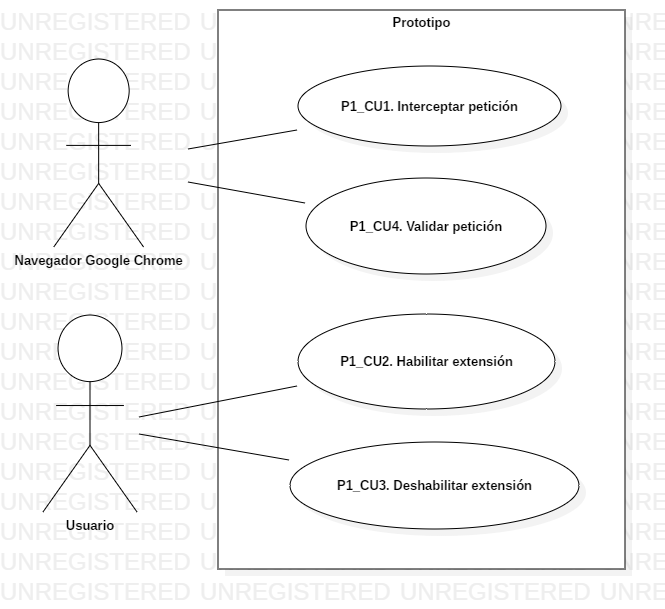
\includegraphics[width=12cm]{./imagenes/UseDiagram_P1v2.png}
						\caption{Diagrama de casos de uso del Prototipo I.}
					\end{center}
				\end{figure}\newpage	
					
			\subsubsection{Descripción de casos de uso.}
			
				%%DESCRIPCIÓN PI_CU1
				\begin{table}[htb]
				\begin{tabular}{ |p{3.5cm}||p{9.5cm}|}
					\hline
					\rowcolor{guindapoli}
					\multicolumn{2}{|c|}{\textbf{\textcolor{white}{Caso de uso: PI\_CU1. Interceptar petición.}}}\\
					\hline
					\rowcolor{azulfuerte}Concepto & Descripción\\
					\hline
					\cellcolor{azulclaro}Actor & 
					Navegador de Google Chrome.\\ 
					\hline
					\cellcolor{azulclaro}Propósito &
					Este caso de uso permite a la extensión interceptar una petición HTTP, realizada por el navegador Google Chrome por medio de algún agente (sistema o usuario) externo a éste.\\
					\hline
					\cellcolor{azulclaro}Entradas &
					Petición HTTP realizada por el navegador.\\
					\hline
					\cellcolor{azulclaro}Salidas &
					Petición HTTP cachada.\\
					\hline
					\cellcolor{azulclaro}Pre-condiciones&
					Algún agente externo (Sistema o usuario) ha ordenado al navegador mandar una petición HTTP.\\
					\hline
					\cellcolor{azulclaro}Post-condiciones&
					La extensión, deberá de interceptar la petición para poder modificarla.\\
					\hline
					\cellcolor{azulclaro}Reglas del negocio&
					-\\
					\hline
					\cellcolor{azulclaro}Errores &
					La petición no se pudo interceptar. \newline La petición no es tipo HTTP.\\					
					\hline
				\end{tabular}
				\caption[DCU: PI\_CU1]{Descripción CU: PI\_CU1}
				\end{table}
				
				\paragraph{... Trayectoria Principal ...}
				\begin{enumerate}
					\item \textbf{\textit{El Usuario}} o \textbf{\textit{El Sistema Externo}} realiza una petición HTTP en el navegador Google Chrome.\\
					\item \textbf{\textit{La Extensión}} intercepta la petición antes de que salga a red.\\
					\item \textbf{\textit{La Extensión}} puede modificar el contenido de la petición. \\
				\end{enumerate}
				\paragraph{... Fin de la Trayectoria Principal ...}
				
				\paragraph{... Trayectoria Alternativa 1 ...}
				\begin{enumerate}
					\item \textbf{\textit{El Usuario}} o \textbf{\textit{El Sistema Externo}} no realiza una petición HTTP en el navegador Google Chrome.\\
					\item \textbf{\textit{La Extensión}} ignora la petición.					
				\end{enumerate}
				\paragraph{... Fin de la Trayectoria Alternativa 1 ...}
				
				\paragraph{... Trayectoria Alternativa 2 ...}
				\begin{enumerate}
					\item \textbf{\textit{El Usuario}} o \textbf{\textit{El Sistema Externo}} realiza una petición HTTP en el navegador Google Chrome.\\
					\item \textbf{\textit{La Extensión}} no puede interceptar la petición antes de que salga a red.\\
					\item \textbf{\textit{La Extensión}} notifica que hubo un error al intentar interceptar la petición. 
				\end{enumerate}
				\paragraph{... Fin de la Trayectoria Alternativa 2 ...}
				
				\newpage
				%%DESCRIPCIÓN PI_CU2
				\begin{table}[htb]
				\begin{center}
				\begin{tabular}{ |p{3.5cm}||p{9.5cm}|}
					\hline
					\rowcolor{guindapoli}
					\multicolumn{2}{|c|}{\textbf{\textcolor{white}{Caso de uso: PI\_CU2. Habilitar extensión.}}}\\
					\hline
					\rowcolor{azulfuerte}Concepto & Descripción\\
					\hline
					\cellcolor{azulclaro}Actor & 
					Usuario.\\ 
					\hline
					\cellcolor{azulclaro}Propósito &
					Este caso de uso, permite al usuario habilitar a la extensión, para que ésta sea capaz de ver todas las peticiones que realiza el navegador.\\
					\hline
					\cellcolor{azulclaro}Entradas &
					Indicación de habilitar extensión, mediante interfaz de usuario.\\
					\hline
					\cellcolor{azulclaro}Salidas &
					Ninguna.\\
					\hline
					\cellcolor{azulclaro}Pre-condiciones&
					El usuario debe de haber instalado la extensión en Google Chrome y haber permitido su ejecución.\\
					\hline
					\cellcolor{azulclaro}Post-condiciones&
					La extensión verá todas las peticiones que realice el navegador.\\
					\hline
					\cellcolor{azulclaro}Reglas del negocio&
					\hyperref[PI_RN1]{PI\_RN1.}\\
					\hline
					\cellcolor{azulclaro}Errores &
					No se puede iniciar la vigilancia de la extensión.\\
					
					\hline
				\end{tabular}
				\caption[DCU: PI\_CU2]{Descripción CU: PI\_CU2}
				\end{center}
				\end{table}
				
				\paragraph{... Trayectoria Principal ...}
				\begin{enumerate}
					\item \textbf{\textit{El usuario}} da click en el ícono de la extensión \textbf{insert icon}.
					\item \textbf{\textit{El usuario}} da click en el botón \textbf{insert button} "Habilitar extensión".
					\item \textbf{\textit{La extensión}} empieza a vigilar las peticiones que se realicen a través del navegador.
				\end{enumerate}
				\paragraph{... Fin de la Trayectoria Principal ...}
				
				\paragraph{... Trayectoria Alternativa 1 ...}
				\begin{enumerate}
					\item \textbf{\textit{El usuario}} da click en el ícono de la extensión \textbf{insert icon}.
					\item \textbf{\textit{El usuario}} da click en el botón \textbf{insert button} "Deshabilitar extensión".
					\item \textbf{\textit{La extensión}} muestra mensaje de error "La extensión ya está deshabilitada".
				\end{enumerate}
				\paragraph{... Fin de la Trayectoria Alternativa 1 ...}
				
				\paragraph{... Trayectoria Alternativa 2 ...}
				\begin{enumerate}
					\item \textbf{\textit{El usuario}} no encuentra el ícono de la extensión \textbf{insert icon}.
				\end{enumerate}
				\paragraph{... Fin de la Trayectoria Alternativa 2 ...}
				
				\newpage
				
				\newpage
				%%DESCRIPCIÓN PI_CU3
				\begin{table}[htb]
				\begin{center}
				\begin{tabular}{ |p{3.5cm}||p{9.5cm}|}
					\hline
					\rowcolor{guindapoli}
					\multicolumn{2}{|c|}{\textbf{\textcolor{white}{Caso de uso: PI\_CU3. Deshabilitar extensión.}}}\\
					\hline
					\rowcolor{azulfuerte}Concepto & Descripción\\
					\hline
					\cellcolor{azulclaro}Actor & 
					Usuario.\\ 
					\hline
					\cellcolor{azulclaro}Propósito &
					Este caso de uso, permite al usuario deshabilitar a la extensión, para que ésta ignore todas las peticiones que se realicen por medio del navegador.\\
					\hline
					\cellcolor{azulclaro}Entradas &
					Indicación de deshabilitar extensión, mediante interfaz de usuario.\\
					\hline
					\cellcolor{azulclaro}Salidas &
					Ninguna.\\
					\hline
					\cellcolor{azulclaro}Pre-condiciones&
					El usuario debe de haber instalado la extensión en Google Chrome y haber permitido su ejecución.\\
					\hline
					\cellcolor{azulclaro}Post-condiciones&
					La extensión dejará de ver todas las peticiones que realice el navegador.\\
					\hline
					\cellcolor{azulclaro}Reglas del negocio&
					\hyperref[PI_RN1]{PI\_RN1.}\\
					\hline
					\cellcolor{azulclaro}Errores &
					No se puede detener la vigilancia de la aplicación.\\
					\hline
				\end{tabular}
				\caption[DCU: PI\_CU3]{Descripción CU: PI\_CU3}
				\end{center}
				\end{table}
			
				\paragraph{... Trayectoria Principal ...}
				\begin{enumerate}
					\item \textbf{\textit{El usuario}} da click en el ícono de la extensión \textbf{insert icon}.
					\item \textbf{\textit{El usuario}} da click en el botón \textbf{insert button} "Deshabilitar extensión".
					\item \textbf{\textit{La extensión}} deja de vigilar las peticiones que se realicen a través del navegador.
				\end{enumerate}
				\paragraph{... Fin de la Trayectoria Principal ...}
				
				\paragraph{... Trayectoria Alternativa 1 ...}
				\begin{enumerate}
					\item \textbf{\textit{El usuario}} da click en el ícono de la extensión \textbf{insert icon}.
					\item \textbf{\textit{El usuario}} da click en el botón \textbf{insert button} "Habilitar extensión".
					\item \textbf{\textit{La extensión}} muestra mensaje de error "La extensión ya está habilitada".
				\end{enumerate}
				\paragraph{... Fin de la Trayectoria Alternativa 1 ...}
				
				\paragraph{... Trayectoria Alternativa 2 ...}
				\begin{enumerate}
					\item \textbf{\textit{El usuario}} no encuentra el ícono de la extensión \textbf{insert icon}.
				\end{enumerate}
				\paragraph{... Fin de la Trayectoria Alternativa 2 ...}
			    
			    %DESCRIPCION PI_CU4
			    \begin{table}[htb]
				\begin{center}
				\begin{tabular}{ |p{3.5cm}||p{9.5cm}|}
					\hline
					\rowcolor{guindapoli}
					\multicolumn{2}{|c|}{\textbf{\textcolor{white}{Caso de uso: PI\_CU4. Validar petición.}}}\\
					\hline
					\rowcolor{azulfuerte}Concepto & Descripción\\
					\hline
					\cellcolor{azulclaro}Actor & 
					Navegador Google Chrome.\\ 
					\hline
					\cellcolor{azulclaro}Propósito &
					En este caso de uso, la extensión evalua si la petición que se interceptó es alguna página web , o si es simplemente una búsqueda que realizó el usuario en la barra de navegación.\\
					\hline
					\cellcolor{azulclaro}Entradas &
					Petición HTTP realizada por el navegador.\\
					\hline
					\cellcolor{azulclaro}Salidas &
					Petición HTTP cachada.\\
					\hline
					\cellcolor{azulclaro}Pre-condiciones&
					Algún agente externo que ha ordenado al navegador mandar una petición HTTP.\\
					\hline
					\cellcolor{azulclaro}Post-condiciones&
					La extensión evaluará el tipo de petición que se reciba para saber si debe interceptarla o no.\\
					\hline
					\cellcolor{azulclaro}Reglas del negocio&
					\hyperref[PI_RN1]{PI\_RN1.}\\
					\hline
					\cellcolor{azulclaro}Errores &
					La petición no se pudo itnerceptar.\\
					\hline
				\end{tabular}
				\caption[DCU: PI\_CU4]{Descripción CU: PI\_CU4}
				\end{center}
				\end{table}
				
				\paragraph{... Trayectoria Principal ...}
				\begin{enumerate}
					\item \textbf{\textit{El Usuario}} o \textbf{\textit{El Sistema Externo}} realiza una petición HTTP en el navegador Google Chrome.\\
					\item \textbf{\textit{La Extensión}} recibe la petición del usuario o sistema externo.\\
					\item \textbf{\textit{La Extensión}} analiza que tipo de petición recibió.\\
					\item \textbf{\textit{La Extensión}} intercepta la petición si es una petición HTTP o la ignora si es una búsqueda realizada por el usuario en la barra del navegador. \\
				\end{enumerate}
				\paragraph{... Fin de la Trayectoria Principal ...}
				
				\paragraph{... Trayectoria Alternativa 1 ...}
				\begin{enumerate}
					\item \textbf{\textit{El Usuario}} o \textbf{\textit{El Sistema Externo}} no realiza una petición HTTP en el navegador Google Chrome.\\
					\item \textbf{\textit{La Extensión}} ignora la petición.					
				\end{enumerate}
				\paragraph{... Fin de la Trayectoria Alternativa 1 ...}
				
				\paragraph{... Trayectoria Alternativa 2 ...}
				\begin{enumerate}
					\item \textbf{\textit{El Usuario}} o \textbf{\textit{El Sistema Externo}} realiza una petición HTTP en el navegador Google Chrome.\\
					\item \textbf{\textit{La Extensión}} no puede recibir la petición.\\
					\item \textbf{\textit{La Extensión}} notifica que hubo un error al intentar recibir la petición. 
				\end{enumerate}
				\paragraph{... Fin de la Trayectoria Alternativa 2 ...}
				\newpage
				%FIN DE LA DESCRIPCIÓN DE CASOS DE USO
				
			\subsubsection{Diagrama de flujo de datos (DFD).}
    			\begin{figure}[!htb]
    			    \begin{center}
    			        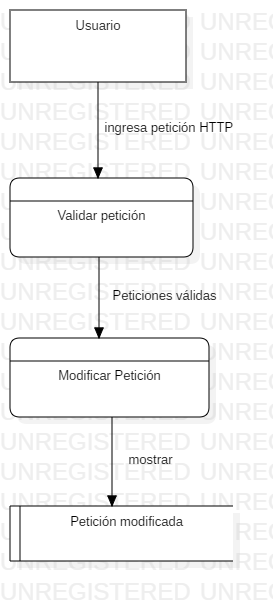
\includegraphics[width=0.5\textwidth]{imagenes/DFD_P1.png}
    			        \caption{Diagrama de flujo de datos del Prototipo 1.}
    				\end{center}
    			\end{figure}
			   
			%\subsubsection{Flujo de datos.}
			\subsubsection{Diagrama de clases.}
				\begin{figure}[!htb]
					\begin{center}
						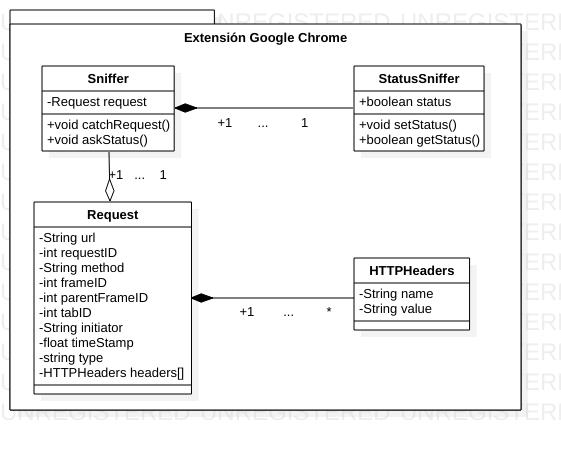
\includegraphics[width=13cm]{./imagenes/DC_P1.png}
						\caption{Diagrama de clases del Prototipo I.}
					\end{center}
				\end{figure}\newpage
				
			\subsubsection{Diagrama de secuencia.}
		    	\begin{figure}[!htb]
				    \begin{center}
			            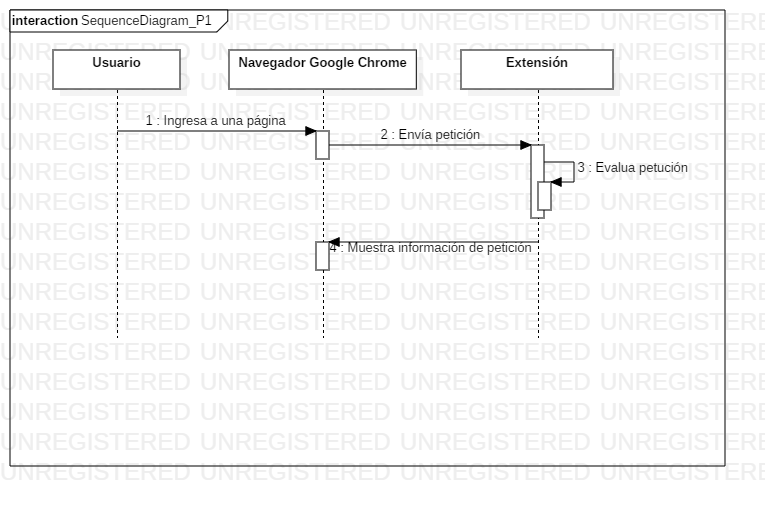
\includegraphics[width=15cm]{./imagenes/SequenceDiagram_P1.png}
				        \caption{Diagrama de secuencia del Prototipo I.}
			        \end{center}
			    \end{figure}
			\subsubsection{Interfaz de usuario.}
			\subsubsection{Requisitos de diseño.}
	%Para agregar una cita en el documento se usa \cite{refKey}, por automático los ordena conforme se van agregando
	\begin{thebibliography}{20}
	    \bibitem{ComparisonAuthenticationMethodsResources} Antonina Komarova, Alexander Menshchikov, “Comparison of Authentication Methods on Web Resources”, St. Petersburg National Research University of Information Technologies, St. Petersburg, Russia, 2016.
		\bibitem{refJavaScript} https://www.dtic.upf.edu/~tnavarrete/fcsig/javascript.pdf 
		\bibitem{refElGranLibro} https://gutl.jovenclub.cu/wp-content/uploads/2013/10/El+gran+libro+de+HTML5+CSS3+y+Javascrip.pdf
		\bibitem{refSeguridadWeb} https://www.seguridad.unam.mx/historico/documento/index.html-id=17
		\bibitem{refRoboIdentidad}
		https://www.seguridad.unam.mx/historico/documento/index.html-id=16?fbclid=IwAR0u8WAXORvBxZ3H-aMzlBhd-6o7g8ycS88eRu7nY1t1XVtCufhEcQ7hWDs
		\bibitem{refSeguridadWebAguilar} Aguilar, A. and Hernández, A. (25 de Abril de 2014). Obtenido de Sugerencias de Seguridad para Sitios Web: http://www.seguridad.unam.mx/documento-id=1143
		
	\end{thebibliography}		
\end{document}

